\section{Method}\label{sec:method}
Our method maintains finite sets of states from which the starts and goals of each training iteration are sampled uniformly at fixed ratios; $\rho^{\mathrm{S}}_e$ and $\rho^{\mathrm{G}}_e$ in Eq.~(\ref{eq:bidirectional}) are the resulting discrete distributions, and we describe the method in terms of these sets.
In the following, we first describe our method's frontier expansion mechanism for the backwards expansion, and how it extends RC's expansion mechanism to provide coverage of the task space and thus the initial distribution. Then we show how the same mechanism can be applied to the forwards expansion by substituting the start state with the goal state. Finally, we combine the two into our main contribution: a bidirectional expansion mechanism that expands the curriculum from both the start and goal states, leading to more sample-efficient and robust learning. An overview of the full method is given in Figure~\ref{fig:method} in the appendix.

% ~2-2.5 pages.
% Schematic Figure 2 (system overview) near the top: \label{fig:method}.
% One sub-headed \paragraph{} per component.
% Equations for the curriculum sampling/scoring rule.
% Algorithm box: uncomment the algorithm packages in main.tex.
% Defer hyperparameters to the appendix (Sec.~\ref{sec:appendix}).


% Overview with a figure
\subsection{Incremental Spatial Expansion}

\paragraph{Exploration:}
Similar to RC~\citep{florensa2017reverse}, we initialize the policy training with valid states obtained from simulating random actions in state space (Figure~\ref{fig:bwd_expansion_1}). After the training iteration, we separate frontier states ($R_{\min} < R < R_{\max}$) and successful states ($R_{\max} \leq R$), where $R = R(\tau, g)$ is the return of a single rollout, i.e., a one-sample estimate of $V^{\pi}(s_0, g)$, and then mix them with fixed ratios to create a balanced training set. % give better arguments here
This set contains mostly states that are neither too hard nor too easy for the current policy, and we call this set the ``mixed'' training set.

When choosing seeds for the next iteration of random walks, we add an additional criterion to enforce coverage of the task space and thus promote convergence to the initial distribution. To do so, we find the spatial frontier (Figure~\ref{fig:bwd_expansion_2}) of the explored state space by (1) sampling a set of random points uniformly from the task space $\mathcal{T}$, (2) computing the nearest neighbor in the
mixed training set for each of the sampled states, and (3) selecting these states as the seeds for the random walks (Figure~\ref{fig:bwd_expansion_3}). Similarly to the Voronoi bias inherent in Rapidly-exploring Random Trees (RRT)~\citep{lavalle2001randomized}, this biases the random walks towards unexplored areas of the task space, as they have a higher probability of being sampled than states in already explored areas.

\begin{figure}[ht]
    \centering
    \begin{subfigure}[t]{0.3\linewidth}
        \centering
        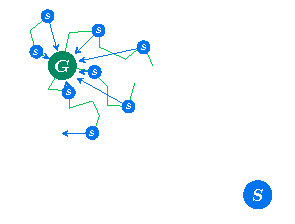
\includegraphics[width=\linewidth]{img/graphics/bwd1.pdf}
        \caption{Starting from the goal, the policy is trained on physically valid initial states ({\color{blue} blue circles}) from random walks ({\color{teal} green lines}) seeded in the goal ({\color{teal} green circle}).}\label{fig:bwd_expansion_1}
    \end{subfigure}
    \hfill
    \begin{subfigure}[t]{0.3\linewidth}
        \centering
        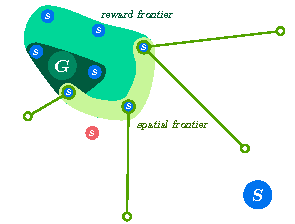
\includegraphics[width=\linewidth]{img/graphics/bwd2.pdf}
        \caption{In addition to the reward frontier ({\color{teal} light green}), the nearest neighbors of random samples from the task space determine the spatial frontier ({\color{orange} yellow circles}).}\label{fig:bwd_expansion_2}
    \end{subfigure}
    \hfill
    \begin{subfigure}[t]{0.3\linewidth}
        \centering
        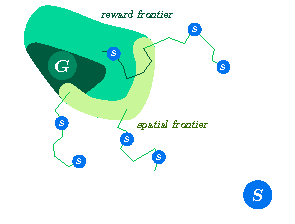
\includegraphics[width=\linewidth]{img/graphics/bwd3.pdf}
        \caption{In the next iteration, the random walks are seeded in the spatial frontier ({\color{orange} yellow circles}), leading to more efficient exploration.}\label{fig:bwd_expansion_3}
    \end{subfigure}
    \caption{Backwards expansion mechanism used in the exploration step.}\label{fig:expansion}
\end{figure}

\paragraph{Exploitation:} In addition to training the policy on unseen states in the exploration step, we also continue training on the mixed training set. This has two effects: (1) training on the reward frontier improves the policy, and (2) training on successful states mitigates catastrophic forgetting. A fixed ratio of training iterations is allocated to this step. If the policy is trained on a parallelized environment, this can be done in parallel with the exploration step, which is the case in our experiments.

Both the exploration and exploitation steps are repeated until the policy is able to solve the task from the initial distribution.


\subsection{Bidirectional Expansion}

\paragraph{Forwards expansion:}
The backwards expansion mechanism described in the previous section can be applied to the forwards expansion by substituting the start state with the goal state. The goal-conditioned policy is trained on initial states sampled from the initial distribution $\rho_0$ and goals sampled from the spatial frontier of the explored state space, i.e., $(s_0 \sim \rho_0,\, g_i)$ rather than $(s_i,\, g^\star)$. The exploration and exploitation steps are then identical, with the minor difference that the random walks are seeded in states that can be reached rather than states from which the goal can be reached.

\paragraph{Bidirectional expansion:} Combining the two expansion mechanisms, we train one shared goal-conditioned policy on both $(s_0 \sim \rho_0,\, g_i)$ and $(s_i,\, g^\star)$, with the training budget split evenly between the two expansions ($\beta = \tfrac{1}{2}$ in Eq.~(\ref{eq:bidirectional})). This leads to a diverse, incrementally expanding curriculum that covers the reachable task space from two directions. As a result, the policy is trained to reach the target goal from a wide range of start states, and to reach a wide range of goals from the initial distribution, leading to more robust policies.

\begin{wrapfigure}{r}{0.3\linewidth}
    \centering
    % \vspace{-\baselineskip} % add again if formatting changes
    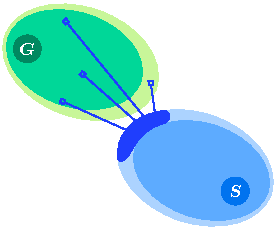
\includegraphics[width=\linewidth]{img/graphics/connect.pdf}
    \caption{The forwards expansion set can be connected to the backwards
        expansion set by sampling from the other mixed training set rather than
        random samples from the task space.}\label{fig:connect}
\end{wrapfigure}
\paragraph{Connecting the two frontiers:} In addition to the bidirectional expansion, we can also connect the two frontiers by replacing the random samples from $\mathcal{T}$ in step (1) of the spatial expansion with samples from the other frontier (Figure~\ref{fig:connect}). For example, when expanding the forwards frontier, we sample states from the mixed training set of the backwards expansion and then find their nearest neighbors in the mixed training set of the forwards expansion. As a result, the seeds of the forwards random walks lie on the side of the forwards set that faces the backwards set, and the intermediate goals grow toward the target goal $g^\star$. Symmetrically, the seeds of the backwards random walks face the forwards set, and the intermediate starts grow toward the initial distribution $\rho_0$.

% \begin{figure}[h]\label{fig:method}
%     \begin{center}
%         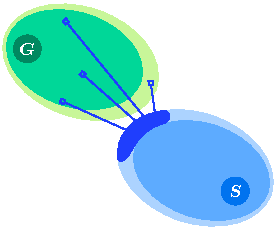
\includegraphics[width=0.3\linewidth]{img/graphics/connect.pdf}
%     \end{center}
%     \caption{The forwards expansion set can be connected to the backwards expansion set by sampling from the other mixed training set rather than random samples from the task space.}\label{fig:connect}
% \end{figure}


This leads to a more sample-efficient exploration, as each expansion moves toward the region the other expansion has already made solvable instead of spreading uniformly over $\mathcal{T}$. This is similar to the RRT-Connect algorithm~\citep{kuffner2000rrt}, where two trees are grown towards each other until they connect.

To promote both even coverage of the task space and the connection of the two frontiers, we sample from both the other frontier and the task space with a fixed ratio, the connect ratio. It balances even coverage of $\mathcal{T}$ against the connection of the two frontiers and is a hyperparameter of our method.